\subsubsection{Valves}

Transient flows in pipe networks may be caused by the closing and opening of valves. In order to describe the transient behaviour of a valves we must define the valve open percentage $\phi(t)$ as a function of time. The valve open percentage is then used to determine the loss coefficient $k$ in the valve resistance equation \eqref{valve_resistance}.

\paragraph{Closing}
 
 The function $\phi(t)$, as shown in figure \ref{fig:valve_closing}, for a valve closure is given by 
\begin{align}\label{valve_closure_function}
\phi(t) = 
\begin{cases} 
\phi_{steady}, &\text{if} \hspace{0.5cm} t \leq t_e \\
\phi_{steady} \left( 1 - \frac{t-t_e}{t_c} \right)^m, &\text{if} \hspace{0.5cm} t_e \leq t \leq t_e + t_c \\
0, &\text{if} \hspace{0.5cm} t \geq t_e + t_c, 
\end{cases}
\end{align} 
where $t_e$ is the event time, $t_c$ is the time taken for the valve to close, $\phi_{steady}$ is the steady state valve open percentage. The exponent $m > 0$ modifies the shape of the closure profile with $m=1$ corresponding to a linear profile. 
 
\begin{figure}
\centering
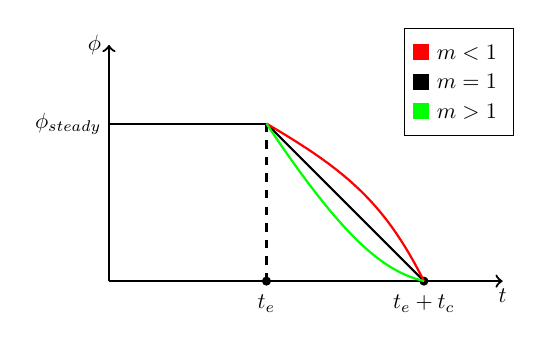
\begin{tikzpicture}[
	scale=1, 
	every node/.style={scale=0.8},
	greennode/.style={shape=rectangle, fill=green, draw=green, minimum size =0.01cm},
	rednode/.style={shape=rectangle, fill=red, draw=red, minimum size =0.01cm},
	blacknode/.style={shape=rectangle, fill=black, draw=black, minimum size =0.01cm},
] 
\draw[thick, ->] (0,0) -- (0,3);
\node[anchor=east] at (0,3) {$\phi$};
\draw[thick, ->] (0,0) -- (5,0);
\node[anchor=north] at (5,0) {$t$};
\node[anchor=north] at (2,-0.08) {$t_e$};
\draw[fill=black] (2,0) circle (0.05cm);
\node[anchor=north] at (4,-0.08) {$t_e + t_c$};
\draw[fill=black] (4,0) circle (0.05cm);
\node[anchor=east] at (0,2) {$\phi_{steady}$};
\draw[thick] (0,2) -- (2,2);
\draw[thick] (2,2) -- (4,0);
\draw[thick, dashed] (2,2) -- (2,0);
\draw[thick, red] (2,2) .. controls (3,1.414) and (3.5,1) .. (4,0);
\draw[thick, green] (2,2) .. controls (3,0.5) and (3.5,0.125) .. (4,0);

\matrix [draw,below left] at (current bounding box.north east) {
  \node [rednode,label=right: {$m < 1$}] {}; \\
  \node [blacknode,label=right: {$m = 1$}] {}; \\
  \node [greennode,label=right: {$m > 1$}] {}; \\
};
\end{tikzpicture} 
\caption{Valve closure. The open percentage $\phi(t)$ goes from $\phi_{steady}$ at time $t_e$ to zero at time $t_e + t_c$, where $t_c$ is the time taken for the valve to close. The exponent $m$ modifies the closure profile, as shown by the red and green curves.}
\label{fig:valve_closing}
\end{figure}

\paragraph{Opening}

{\color{red} TODO Valve opening}